\section{Insert-First-Verfahren} \label{sec:insert-first-verfahren}
% Was ist das Min Dist Verfahren?
    % Nodes werden in der Reihenfolge ihres Auftretens in den Graphen eingefügt
    % Insert-First = dadurch insert-random  
% Wie funktioniert es
    % Ein neuer Graph mit einem Pfad der länge n wird erzeugt
    % Die Nodes des Pfades des Graphen seien Y1,Y2,Y3,Y4...
    % Die erst Node des Pfads wird mit der ersten Node in der Liste der Verfügbaren Nodes befüllt (= Ausgangs-Node)
    % Die zweite Node wird ebenso aus den verfügbaren Nodes angehängt (ist nun an zweiter Stelle)
    % Nun wird durch die restlichen Verfügbaren Nodes iteriert
    % Node X sei Gegenstand des momentanen Iterationdurchlaufs 
    % Für X wird beginnend mit Y2 die Distanz zwischen Yn-1 und X + Distanz zwischen Yn und X errechnet
    % resultierend aus diesen Berechnungen wird die beste Stelle gesucht, um X in den Pfad einzufügen
% Teile des Quellcodes zeigen
\subsection{Funktionsweise}
Das Insert-First-Verfahren ist ein heuristischer Lösungsansatz des \ac{TSP}s, bei dem das Betrachten der Knoten zum Aufbau eines Graphen in zufälliger Reihenfolge, bzw. in der Reihenfolge ihrer Erzeugung geschieht.
Dabei wird zu einem Zeitpunkt genau ein Knoten betrachtet und an der für ihn bestmöglichen Stelle in den bereits bestehenden Graphen eingefügt.


\begin{algorithm}[H]
    \caption{Insert-First-Algorithmus}
    \label{alg:insert-first}
    \begin{algorithmic}[1]
        \Require Graph $G$, Pfad $P$
        \Require $G = k_1,k_2,\ldots,k_n$, $n > 2$
        % \ENSURE $G$ length $> 2$
        \State $p_1 \gets k_1$
        \Comment Setzen der ersten beiden Knoten
        \State $p_2 \gets k_2$
        \For{$a \gets 3$, $a \leq n$, $a \gets a + 1$}
            \State $j_S \gets -1$
            \Comment Index der geringsten Distanz
            \State $d_S$ $\gets -1$
            \Comment Geringste Distanz
            \For{$b \gets 1$, $b \leq m$, $b \gets b +1$} 
                \State $d_C \gets$ \textsc{mergeAt}($P$, $b$, $k_a$) \textsc{distance}
                \Comment Gesamtdistanz, wenn $k_a$ am Index $b$ in $P$ eingefügt werden würde (siehe Alg. \vref{alg:merge-node-into-path})
                %simulateMerge($P$, $b$, $G_a$).getTotalDistance()
                \If{$j_S =-1$ \textbf{or} $d_C < d_S$}
                    \State $d_S$ $\gets$ $d_C$
                    \Comment Kürzeste Distanz wird übernommen
                    \State $j_S \gets b$
                    \Comment Und ihr Index
                \EndIf
            \EndFor
            \State $P \gets$ \textsc{mergeAt}($P$, $j_S$, $k_a$)
            \Comment $k_a$ wird am Index $j_S$ in $P$ eingefügt
        \EndFor \\
        \Return new Graph($P$)
        \Comment Graph mit Pfad $P$ wird zurückgegeben
    \end{algorithmic}
\end{algorithm}
% Zu Beginn des Insert-First-Verfahrens wird ein neuer Graph erzeugt, welcher als Eingabewerte eine Liste mit den Knoten $k_1, k_2,  \ldots ,k_n$, hier bezeichnet als \lstinline{nodes} und der Länge $n$ erhält.
Als Eingabe erhält der Algorithmus einen Graphen mit einer ungeordneten Liste von $n$ Knoten $k_1,k_2,\ldots,k_n$ mit $n > 2$.
Der Algorithmus erzeugt einen Pfad $P$, in dem die Knoten des Graphs $G$ eingefügt und angeordnet werden.
Nach vorheriger Definition kann jede gefüllte Position $p_k$ im Pfad $P$ mit einem Knoten $k_l$ des Graphs $G$ gleichgesetzt werden.
Es gilt also $\forall p \in G$.
Wenn beispielsweise:
$$G = k_1,k_2,k_3,k_4$$
und
$$P=p_1,p_2,p_3 \textrm{ mit }p_1=k_1,p_2=k_4,p_3=k_2$$
dann
$$P=k_1,k_4,k_2$$
Nun wird $k_1$, der erste Knoten aus der übergebenen Liste, in den Pfad des Graphs an erster Stelle, $p_1$, eingefügt. 
Dies geschieht so oder ähnlich bei allen Verfahren, um einen statischen Ausgangspunkt zu gewährleisten und somit vergleichbare Ergebnisse zu erzielen.
Anschließend wird noch der zweite Knoten $k_2$ and $P$ angehängt.

% \begin{lstlisting}[caption={Zuweisung des ersten und zweiten Knotens}]
% path[0] = nodes[0];
% path[1] = nodes[1];  
% \end{lstlisting}

Das Vorgehen für das Einfügen der restlichen Knoten lässt sich wie folgt beschreiben: 
Sei $G$ ein Graph mit einer ungeordneten Menge von $n$ Knoten  $k_1,k_2,\ldots,k_n$ und bereits teilweise befülltem Pfad $k_1,\ldots,k_m$ mit $m \geq 2$ und $m < n$.
Die Knoten, die noch eingefügt werden müssen, werden in der Reihenfolge ihres Auftretens in der übergebenen Liste in den Graphen eingefügt, womit der als nächstes einzufügende Knoten immer $k_{i}$ mit $i = m + 1$ ist.
\\
Um die beste Stelle zu ermitteln, in die $k_i$ eingefügt werden soll, wird für jeden möglichen Index, also jede mögliche Stelle, die Gesamtdistanz des entstehenden Graphen berechnet. 
% Aus den so berechneten Möglichkeiten wird die mit der geringsten Distanz vermerkt und ausgewählt.
% % Um die Stelle zu ermitteln, in die $k_i$ eingefügt werden soll, müssen die Distanzen zu Vorgänger und Nachfolger berechnet und die geringste Entfernung ermittelt werden. 
% % Hierzu wird durch die Knoten beginnend mit $k_2$ bis $k_{m+1}$ iteriert. Dabei sei $k_j$ der Knoten des aktuellen Iterationdurchlaufs. 
% % Nun wird die Distanz zwischen $k_{j-1}$ und $k_i$ mit der Distanz zwischen  $k_{j}$ und $k_i$ addiert. Hierbei muss beachtet werden, dass bei der Betrachtung von $k_{j=m+1}$ keine wirkliche Distanz zu $k_i$ errechnet werden kann, da nur $m$ Knoten im Graphen sind. Stattdessen wird angenommen, dass die Distanz 0 beträgt, sodass ein Anfügen an das Ende des Graphen simuliert wird.
% \\
% In Java Quellcode bedeutet dies konkret:
% \begin{lstlisting}[caption={Ermittlung der Distanzen}, label={lst:distjava}]
% double currentDistance = 
%     ((path[j] != null) ? distances.getDistanceById(path[j], nodes[i]) : 0)
%     + distances.getDistanceById(path[j - 1], nodes[i]);

% \end{lstlisting}
Das niedrigste Ergebnis dieser Möglichkeiten wird zusammen mit dem dazugehörigen Index $j$ vermerkt. 
Nachdem die niedrigste Distanz für $k_i$ errechnet wurde kann anhand des Index' der Knoten an der bestmöglichen Stelle in den Graphen eingefügt werden. 
Einfügen bedeutet hier, dass alle Knoten, deren Index gleich oder höher $j$ ist um einen Platz nach hinten verschoben werden. 
Nachdem alle Knoten auf diese Weise verschoben wurden, kann $k_i$ an der Stelle $j$ eingefügt werden, ohne, dass andere Knoten verloren gehen. 
% \begin{lstlisting}[caption={Einfügen von Knoten in einen bestehenden Graph}, label={code:mergeIntojava}]
% private static Node[] mergeNodeIntoGraph(Node[] path, Node node, int index) {
%     for (int i = path.length - 2; i >= index; i--) {
%         path[i + 1] = path[i];
%     }
%     path[index] = node;
%     return path;
% }
% \end{lstlisting}
Beispielhaft sähe das mit den vorher festgelegten Bezeichnungen wie folgt aus: 
% \begin{addmargin}[1em]{2em}
$$P= k_1, k_2, k_4, k_3 \textrm{ und } k_{i = 5}$$ 
% \end{addmargin}
Durch das ermitteln der Gesamtdistanzen in Abhängigkeit zu den möglichen Einfügestellen wird bekannt, dass $k_{i=5}$ mit dem Index $j=4$, also zwischen $k_4$ und $k_3$ bestmöglich eingefügt werden kann, was zu einem Pfad der Form
% \begin{addmargin}[1em]{2em}
$$P=k_1, k_2, k_4, k_5, k_3$$
% \end{addmargin}
führt.
ein Algorithmus, der das Einfügen von Knoten in einen Pfad nach vorherig beschriebener Art implementiert findet sich unter Algorithmus \vref{alg:merge-node-into-path}.

\subsection{Zeitkomplexität}\label{sec:time-comp-first}
Analysiert man den Insert-First-Algorithmus nach seiner Zeitkomplexität lassen sich, in Verbindung mit seinen Ergebnissen, die im Abschnitt \vref{sec:inserst-first-erg} diskutiert werden, Aussagen über seine Effizienz treffen.
\\
Die äußere Iteration beginnend in Zeile 3 des Algorithmus sei hier $I_a$ und die innere beginnend in Zeile 6 $I_b$.
$I_a$ wird, bedingt durch die Abbruchbedingung $a\leq n$ und das Inkrementieren von $a$ um $1$ nach jeder Iteration $n-2$ mal durchlaufen.
Die Laufzeit von $I_b$ ist abhängig von $m$, der Menge der Elemente des Pfads $P$.
Da in jedem Iterationsdurchlauf ein Element in $P$ eingefügt wird, berechnet sich $m$ in einem Iterationsschritt mit $m=a-1$.
Für eine Funktion $f(n)$, welche die Komplexität des Algorithmus in Abhängigkeit zur Eingabemenge in der Form $f: \mathbb{N} \rightarrow \mathbb{N}$ abbildet, lässt sich also sagen
$$f(n) = \sum_{a = 3}^n m_a$$
$$f(n) = \sum_{a=3}^n a - 1$$
$$f(n) = \frac{(n-1)\cdot (n-2)}{2}-1$$
Womit sich ergibt, dass der Algorithmus eine quadratische Laufzeit der Form
$$f(n) = O(n^2)$$
hat.
Daraus lässt sich ablesen, dass die Laufzeit des Algorithmus zwar nicht exponentiell zur Eingabemenge, aber wenigstens noch quadratisch steigt.
Besser wäre hier ein logarithmisches Verhalten, da Algorithmen dieser Art besser für große Eingabemengen Skalieren.\autocite[S. 9ff.]{Gurski.2010}


\subsection{Ergebnisse und Schwächen} \label{sec:inserst-first-erg}
Bevor einige durch den Algorithmus generierte Beispiele betrachtet werden, wird hier das Szenario dieser und aller folgender Beispiele, es sei denn ist anderes angegeben, beschrieben.
Alle gezeigten Knoten befinden sich auf einem zweidimensionalem Fläche mit den Maßen zehn mal zehn \ac{LE}.
Folglich kann jedem Knoten eine X- und Y-Koordinate zwischen jeweils null und zehn zugeordnet werden. 
Dementsprechend bewegen sich auch die Gesamtdistanzen er gezeigten Graphen in dieser Größenordnung.
Weiterhin werden aus Gründen der Übersichtlichkeit für den Großteil der folgenden Beispiele nur Graphen mit fünf Knoten betrachtet.
\\\\
Bei dem Einsatz des oben beschriebenen Algorithmus kommt es zu Ergebnissen, die in ihrer Qualität nah an die optimale Lösung herankommen, teilweise aber auch weit von ihr abweichen können.  

\begin{figure}[H]
    \begin{center}
        \subfloat[$m = 2$\label{subfig:insert-first-BAD-m2}]{%
        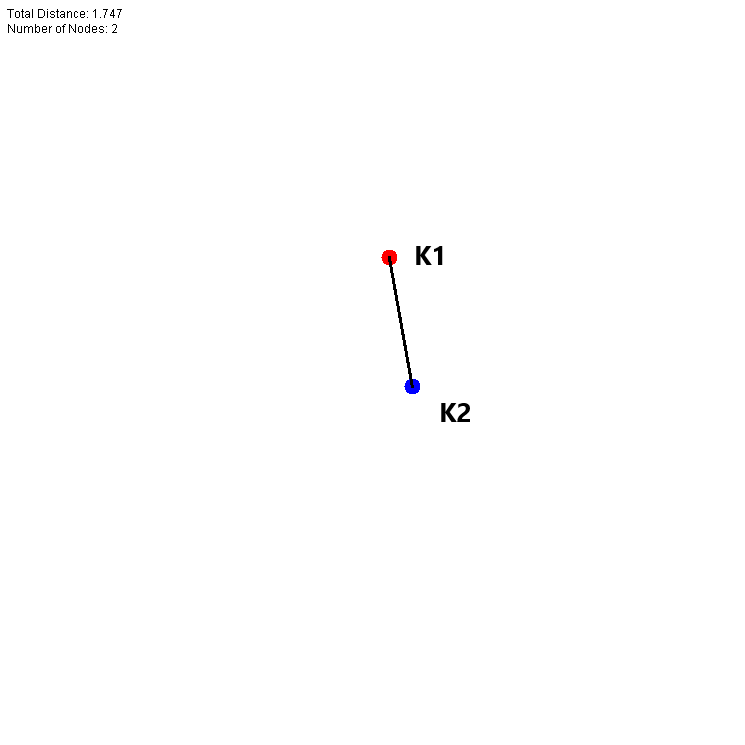
\includegraphics[width=0.35\textwidth]{./Bilder/insertFirst/insert_first_BAD_ex_1.PNG}
        }
        \hfil
        \subfloat[$m = 3$\label{subfig:insert-first-BAD-m3}]{%
        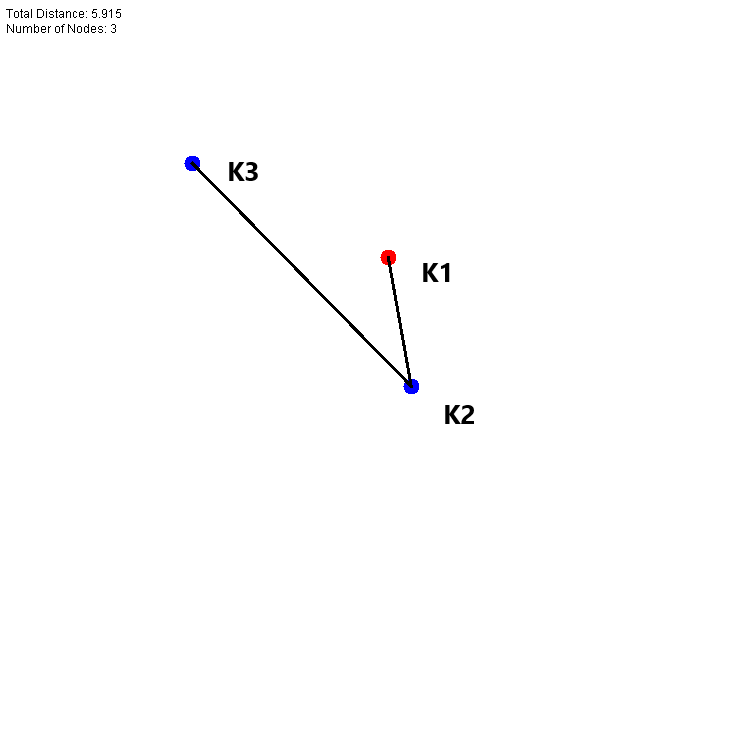
\includegraphics[width=0.35\textwidth]{./Bilder/insertFirst/insert_first_BAD_ex_2.PNG}
        }\\
%     \end{center}
% \end{figure}
% \begin{figure}\ContinuedFloat
%     \begin{center}
        \subfloat[$m = 4$\label{subfig:insert-first-BAD-m4}]{%
        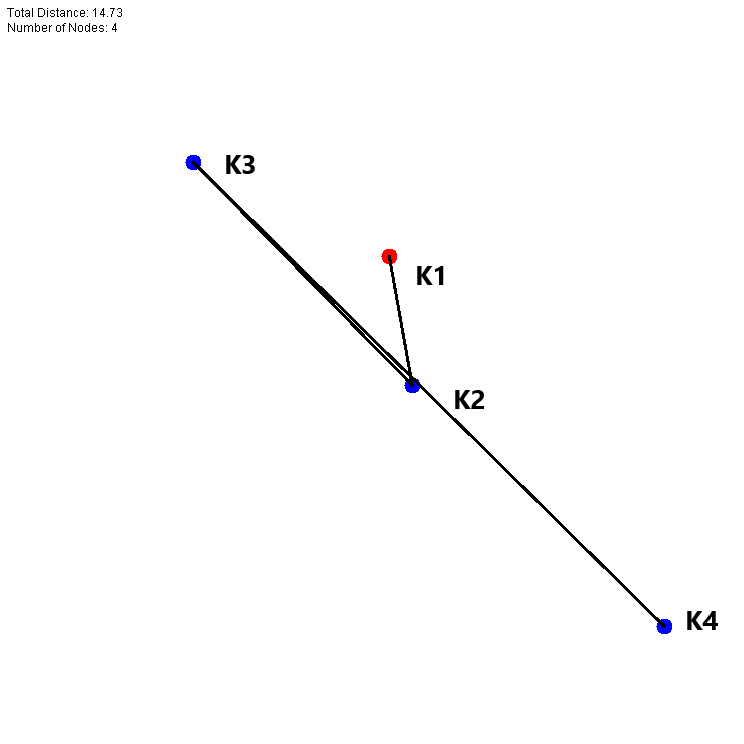
\includegraphics[width=0.35\textwidth]{./Bilder/insertFirst/insert_first_BAD_ex_3.PNG}
        }
        \hfil
        \subfloat[$m = 5$\label{subfig:insert-first-BAD-m5}]{%
        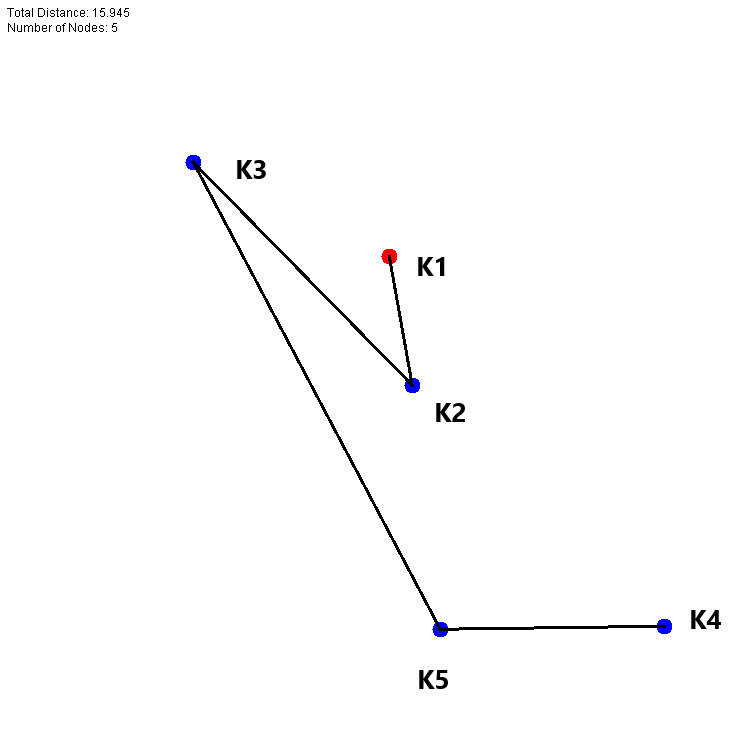
\includegraphics[width=0.35\textwidth]{./Bilder/insertFirst/insert_first_BAD_ex_4.PNG}
        }
        \caption{Insert-First führt zu schlechtem Ergebnis}
        \label{fig:insert-first-bad}
    \end{center}
\end{figure}

% TODO: Alle Schritte/Bilder in den Anhang
Alle gezeigten Bilder sind in größer im Anhang zu finden (Abbildung A.1 im Anhang).\\
Auf \vref{subfig:insert-first-BAD-m4} lässt sich erkennen, dass das Einfügen des vierten Knoten $k_4$ nicht optimal geschieht. 
Besser für $m = 4$ wäre hier der Pfad 
% \begin{addmargin}[1em]{2em}
    $$P=k_1, k_3, k_2, k_4$$
    % \end{addmargin}
Dieser wird allerdings nicht durch das Insert-First-Verfahren gebildet, da dies eine Änderung des bereits erzeugten Graphen in \vref{subfig:insert-first-BAD-m3} erfordern würde. 
Dies ist jedoch nicht möglich, da $k_4$ nur zwischen bereits im Pfad des Graphen vorhandenen Knoten eingefügt werden kann, sodass der schlussendlich generierte Graph eine Gesamtlänge von 15,945 \ac{LE} hat.
Hier lässt sich auch das grundlegende Problem des Algorithmus erkennen: Das Erstellen einer Route ohne vorherige Betrachtung der Gesamtheit der Knoten. 
Einzelne Abschnitte des Graphen können optimal erzeugt werden, wie beispielsweise im Schritt von \vref{subfig:insert-first-BAD-m2} zu \vref{subfig:insert-first-BAD-m3}. 
Andere hingegen, wie vorher erwähnt, nicht. 
Grund hierfür ist die alleinige Betrachtung des Knotens $k_i$. 
Spezifischer bedeutet das, dass das frühe Einfügen von Knoten in den Pfad später zu Komplikationen führen kann, da es objektiv besser gewesen wäre einen anderen Knoten früher einzufügen.
Am konkreten Beispiel führt die generierte Reihenfolge von 
% \begin{addmargin}[1em]{2em}
    $$P=k_1, k_2, k_3 \textrm{ für } m=3$$
    % \end{addmargin}
in \vref{subfig:insert-first-BAD-m3} dazu, dass $k_4$ nur unter einen vergleichsweise großen Gesamtdistanzzuwachs in den Graphen eingefügt werden kann. 
\\\\
Konträr zu diesem schlechten Beispiel ist der Insert-First-Algorithmus auch in der Lage gute bis optimale Ergebnisse zu generieren. 

\begin{figure}[H]
    \begin{center}
        \subfloat[$m = 2$\label{subfig:insert-first-GOOD-m2}]{%
        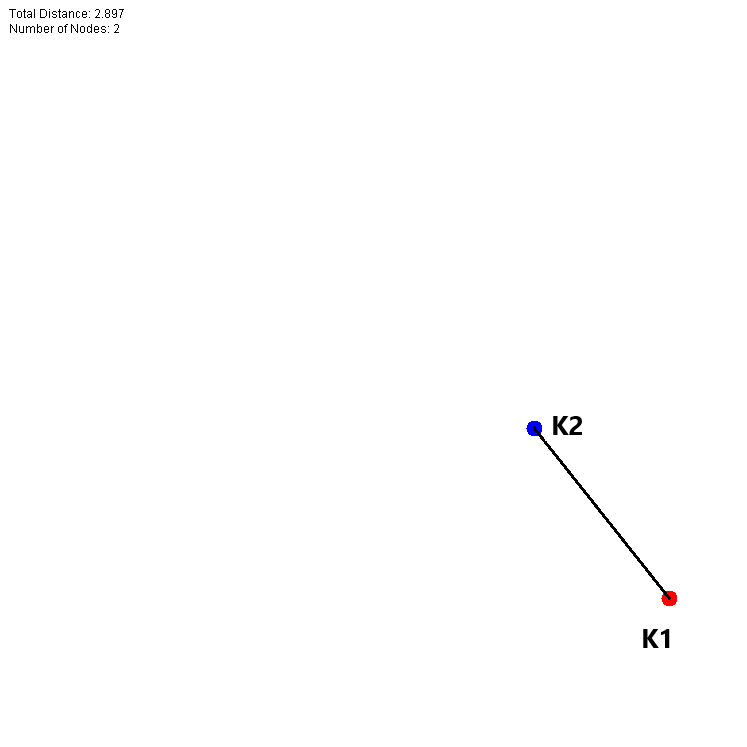
\includegraphics[width=0.35\textwidth]{./Bilder/insertFirst/insert_first_ex_1.PNG}
        }
        \hfil
        \subfloat[$m = 3$\label{subfig:insert-first-GOOD-m3}]{%
        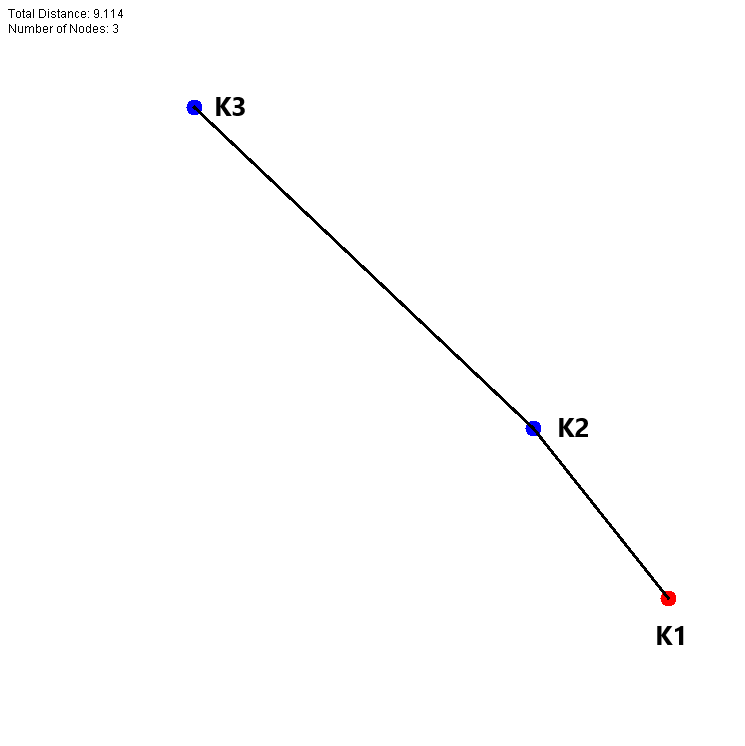
\includegraphics[width=0.35\textwidth]{./Bilder/insertFirst/insert_first_ex_2.PNG}
        }\\
%     \end{center}
% \end{figure}
% \begin{figure}
%     \begin{center}\ContinuedFloat
        \subfloat[$m = 4$\label{subfig:insert-first-GOOD-m4}]{%
        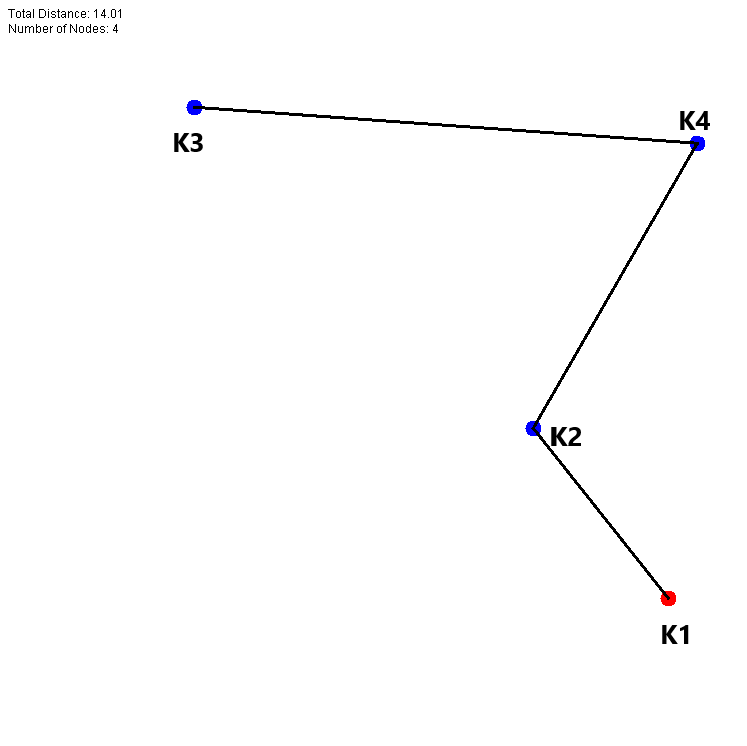
\includegraphics[width=0.35\textwidth]{./Bilder/insertFirst/insert_first_ex_3.PNG}
        }
        \hfil
        \subfloat[$m = 5$\label{subfig:insert-first-GOOD-m5}]{%
        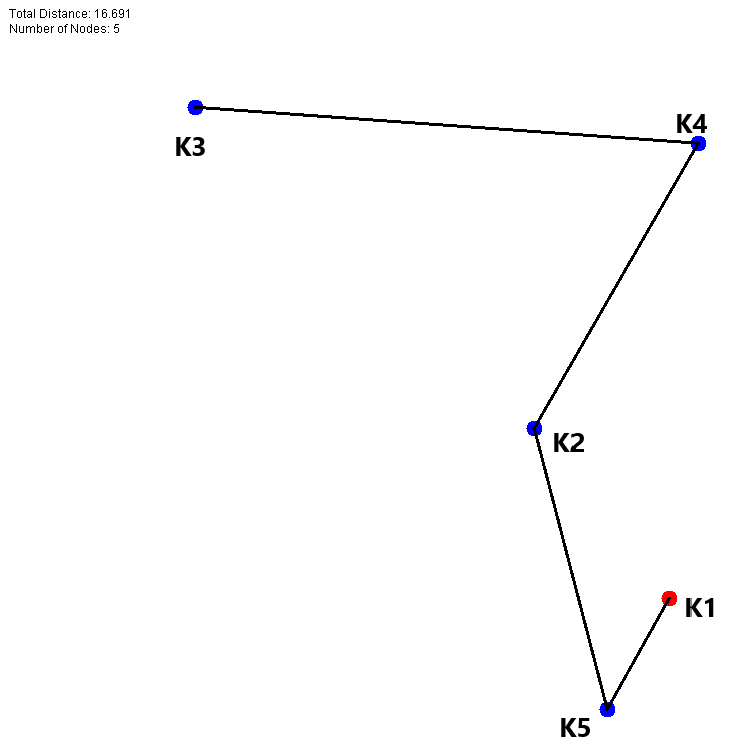
\includegraphics[width=0.35\textwidth]{./Bilder/insertFirst/insert_first_ex_4.PNG}
        }
        \caption{Insert-First führt zu guten Ergebnis}
        \label{fig:insert-first-good}
    \end{center}
\end{figure}
Alle gezeigten Bilder sind in größer im Anhang zu finden (Abbildung A.2 im Anhang).\\
% TODO: Alle Schritte/Bilder in den Anhang
% Alle gezeigten Bilder sind in größer im Anhang zu finden (Abbildung \vref{app:fig:insert-first-GOOD-example-full}).
% \\
Am Beispiel in \vref{fig:insert-first-good} lässt sich erkennen, wie der Insert-First-Algorithmus einen optimalen Pfad mit den gegebenen Knoten generiert. 
Gerade im Schritt von \vref{subfig:insert-first-GOOD-m4} zu \vref{subfig:insert-first-GOOD-m5} ist ein funktionierendes und korrektes Einfügen des Knotens in den Graphen zu sehen, bei dem der Anstieg der Gesamtdistanz der Route sehr gering gehalten wird. 
Hier wird der aktuelle Knoten mit geringem Zuwachs der schlussendlichen Gesamtdistanz in den Graphen eingefügt, sodass die Gesamtdistanz zum Ende bei 16,691 \ac{LE} liegt.
Die ist zwar höher als das vorherige schlechte Beispiel, liegt aber in den Positionen der einzelnen Knoten begründet.
\\\\
Für die Bewertung des Algorithmus müssen also beide Seiten betrachtet werden. 
Zwar ist Insert-First in der Lage eine gute oder auch optimale Route zu erstellen, allerdings beeinflusst die Reihenfolge der Betrachtung der Knoten stark die Qualität des Endergebnisses und kann zu suboptimalen Resultaten führen.


